\chapter{Erros comuns em documentos}
\label{erros-comuns-capitulo}

\section{Erros comuns em documentos}
\label{erros-comuns}

% Não colocar nada aqui pois é uma demonstração de erro comum

\subsection{Subseção sem texto entre o item anterior}
\label{erros-comuns-sub1}

\newcommand{\errado}[1]{\textbf{\textcolor{red}{#1}}}
\newcommand{\certo}[1]{\textbf{\textcolor{ForestGreen}{#1}}}
% Para não confundir com os exemplos de certo e errado não são colocados os pontos e ponto e virgula dos itens
\newcommand{\erradocerto}[3]{\item #1 :\begin{itemize}
    \item \errado{#2}
    \item \certo{#3}
\end{itemize}}
\newcommand{\erradoerradocerto}[4]{\item #1 :\begin{itemize}
    \item \errado{#2}
    \item \errado{#3}
    \item \certo{#4}
\end{itemize}}


Essa seção \autoref{erros-comuns} demonstra alguns dos erros mais comuns que percebemos em trabalhos de alunos. Alguns itens errados são apresentados em \errado{vermelho} e corretos em \certo{verde}, mas devido a formatação dos links pode haver uma variação.

A lista de itens demonstra alguns erros:

\begin{itemize}
    \item \errado{passagem de um item para outro sem texto} como é possível observar entre  \autoref{erros-comuns-capitulo} e \autoref{erros-comuns} e também entre \autoref{erros-comuns} e \autoref{erros-comuns-sub1};
    
    item \errado{itens com pouco texto} como a \autoref{erros-comuns-sub-pequena1} e a \autoref{erros-comuns-sub-pequena2}, cada item deve ter um volume de texto que justifique sua existência;
        
    \item \errado{utilizar o mesmo nome para seções / capítulos como \autoref{erros-comuns-capitulo} e \autoref{erros-comuns}};
        
    \item definições de referências incompletas, a referência \citeonline{ETAL4} está definida faltando cidade, observe que na lista de referencias aparece \errado{[S.l.]} que indica Sem Local, pois a ABNT exige a indicação de local para livros;
        
    \erradocerto{não utilizar o sistema de siglas / glossário para definições especificas,ver \autoref{siglas-glossario}}{IFSP}{\acs{ifsp}}
    
    \erradoerradocerto{utilizar o formato de citação errada, ver \autoref{referencias}}{de acordo com \cite{alcarde1996} ...}{de acordo com \citeauthor{alcarde1996} ...}{de acordo com \citeonline{alcarde1996}...}

% NBR 10520:2002 ver exemplos em 6.1.5
    \erradocerto{erro ao citar em final do paragrafo, o ponto final fica após a citação }{texto.\cite{alcione1988}} {texto \cite{alcione1988}. }


    \erradocerto{utilizar o formato de citação errada em fontes, ver \autoref{referencias}}{Fonte: \cite{alcarde1996}}{Fonte: \citeonline{alcarde1996}}

    \erradocerto{ignorar que após uma macro pode ser necessário incluir um espaço forçado}{o \LaTeX permite...}{o \LaTeX\ permite...}

    \erradocerto{não utilizar palavras em português onde for possível}{o dispositivo mobile}{o dispositivo móvel}

    \erradocerto{não utilizar melhores palavras, algumas palavras chegaram a ser incorporadas a língua portuguesa mas existem palavras melhores e que podem ser utilizadas e as vezes com resultado mais claro}{deletar - postagem}{excluir - publicação}

    \erradocerto{Utilização do tempo verbal incorreto, a escrita do documento muitas vezes inicia antes da finalização, mas o leitor recebe o documento depois do trabalho finalizado}{será desenvolvido - será apresentado}{foi desenvolvido - é apresentado}

    \item \erradocerto{não representar as unidades de forma correta}{3.20 ghz}{3.20 GHz}

    \erradocerto{não ser consistente com os formatos e precisões}{o primeiro tem \emph{clock} de 3.20 GHz e segundo 1.8 GHz}{o primeiro tem \emph{clock} de 3.20 GHz e segundo 1.80 GHz}

    \erradocerto{não referenciar ilustrações da forma correta}{a tabela \ref{tabela-correta-equipamento} ...}{a \autoref{tabela-correta-equipamento} ...}
    
    \item não referenciar uma ilustração no texto. Toda ilusração deve ser referenciada no texto;
    
    \erradocerto{não referenciar corretamente sequencias de ilustrações}{nas \autoref{tab-exemplo} até \autoref{tabela-correta-servicos}}{nas Tabelas de \ref{tab-exemplo} até \ref{tabela-correta-servicos}}

    \erradocerto{deixar referencia jogada sem fazer parte do texto}{durante o projeto foram registradas as métricas. \autoref{tabela-correta-servicos}}{a \autoref{tabela-correta-servicos} apresenta os valores das métricas levantadas durante o projeto.}

    \item \errado{incluir dentro do seu texto um documento ou manual que pode ser referenciado e facilmente acessado pelo leitor}, \certo{faça a citação correta referenciando o documento original}.

    \item \errado{não utilizar o mesmo formato para escrever a mesma coisa}, ex. \textbf{Acme}, \textbf{ACME}, \textbf{acme}, se esse é o nome da sua equipe defina uma macro e utilize sempre da mesma forma;
    
    \item \errado{não utilizar imagens vetorizadas} para obter a melhor qualidade, ver \autoref{sec_figuras};
    
    \item \errado{não seguir as dicas de textos} disponíveis em \url{https://dicas.ivanfm.com/aulas/textos/};
    
    \item \errado{não seguir as dicas de revisão} disponíveis em \url{https://dicas.ivanfm.com/aulas/textos/revisao-de-textos.html};
    
    \item \errado{não formatar corretamente tabelas} como indicado na \autoref{sub-erros-tabelas};

    \item \errado{tentar posicionar ilustrações em locais específicos} (ex abaixo do texto), o correto é referenciar a ilustração no texto e deixar o \LaTeX\ posicionar de acordo com a disponibilidade de espaço no documento, mas você deve recomendar que o local da definição seja prioritário, ver \autoref{elementos-nao-textuais}.
    
\end{itemize}


\subsection{Subseção com texto pequeno 1}
\label{erros-comuns-sub-pequena1}
\errado{Uma frase única indicando basicamente o que o título da seção é}.

\subsection{Subseção com texto pequeno 2}
\label{erros-comuns-sub-pequena2}
\errado{Mais uma paragrafo único indicando basicamente o que o título da seção é, provavelmente isso poderia ir para o glossário, ver \autoref{siglas-glossario}}, uma regra simples para seguir é \certo{se uma seção não tiver pelo menos 3 (três) parágrafos, provavelmente essa informação não precisa de uma seção especifica e pode fazer parte de outra seção}.


\subsection{Subseção sobre erros em tabelas e quadros}
\label{sub-erros-tabelas}
A \autoref{tabelas-e-quadros} demonstra como devemos formatar corretamente tabelas e quadros, a \autoref{tabela-errada} mostra diversos erros comuns que encontramos em tabelas e quadros, e as tabelas \ref{tabela-correta-equipamento} e \ref{tabela-correta-servicos} mostram os mesmos dados apresentados de uma forma correta. Uma tabela formatada corretamente permite a leitura e comparação dos dados de forma mais fácil. Observe a lista de erros da \autoref{tabela-errada} :


\begin{itemize}
    \item \errado{formatação de bordas como um quadro e não como tabela};
    \item \errado{Utilizar \index{longtable}longtable sem necessidade quebrando um quadro ou tabela que poderia ser apresentado em uma única página};
    \item \errado{não limitar tamanho de coluna que tem dados grandes de forma a estourar o espaço disponível};
    \item \errado{números não estão alinhados a direita};
    \item \errado{itens sem ordem especifica}, \certo{os itens devem vir em uma ordem lógica ou ordem alfabética};
    \item \errado{inconsistência de precisão, em uma célula o valor tem duas casas decimais e em outras não possuem casas decimais};
    \item \errado{mistura de dados de situações diferentes, custo único e custo mensal};
    \item \errado{repetição do R\$ mesmo tendo ele no título da coluna}.
\end{itemize}

\begin{table}[thb]
\centering
\ABNTEXfontereduzida
\caption{A tabela formatada de forma errada}
\label{tabela-errada}
\begin{tabular}{|l|c|l|l|}
\hline
\thead{Equipamento/Serviço} & \thead{Valor Unitário R\$} & \thead{Quantidade} & \thead{Valor Total R\$} \\ \hline
Teclado     & R\$60          & 2          & R\$120     \\ \hline
Monitor     & R\$:600          & 2          & R\$ 1200,00     \\ \hline
Internet     & R\$220          & 1          & R\$ 220     \\ \hline
Texto muito grande que deveria gerar quebra     & R\$120          & 1          & R\$ 120     \\ \hline
\end{tabular}
\end{table}

\begin{table}[]
\centering
\ABNTEXfontereduzida
\caption{A tabela errada agora formatada corretamente (custos de compra)}
\label{tabela-correta-equipamento}
\begin{tabular}{m{8.0cm}|r|r|r}
\hline
\thead{Equipamento} & \thead{Valor\\Unitário\\R\$} & \thead{Quantidade} & \thead{Valor\\Total\\ R\$} \\ \hline
Monitor     & 600,00          & 2          & 1200,00     \\ \hline
Teclado     & 60,00          & 2          & 120,00     \\ \hline
Texto muito grande que deveria gerar quebra     & 220,00          & 1          & 220,00     \\ \end{tabular}
\legend{Fonte: Os autores}
\end{table}

\begin{table}[]
\centering
\ABNTEXfontereduzida
\caption{A tabela errada agora formatada corretamente (custos mensais)}
\label{tabela-correta-servicos}
\begin{tabular}{l|r|r|r}
\hline
\thead{Serviço} & \thead{Valor Unitário R\$} & \thead{Quantidade} & \thead{Valor Mensal R\$} \\ \hline
Internet     & 120,00          & 1          & 120,00     \\ \hline
\end{tabular}
\legend{Fonte: Os autores}
\end{table}




Em quadros pequenos detalhes podem fazer uma grande diferença na apresentação de informação, como pode ser observado nos quadros \ref{quadro-poluido} e \ref{quadro-poluido-limpo} :

\begin{itemize}
    \item \errado{O \autoref{quadro-poluido} foi montado com textos que não facilitam a leitura};
    \item \certo{O \autoref{quadro-poluido-limpo} apresenta a mesma informação de forma mais limpa e facilitando a leitura}.
\end{itemize}



\begin{quadro}[thb]
\centering
\ABNTEXfontereduzida
\caption{Quadro de Atividades poluído, difícil de ler }
\label{quadro-poluido}
\begin{tabular}{|l|c|c|c|c|}
\hline
\thead{Responsável} & \thead{Atividade 1} & \thead{Atividade 2} & \thead{Atividade 3} & \thead{Atividade 4} \\
\hline
%
Pessoa 1 & SIM         & NÃO         & NÃO         & SIM         \\
\hline
Pessoa 2 & SIM         & NÃO         & SIM         & NÃO         \\
\hline
Pessoa 3 & NÃO         & SIM         & NÃO         & NÃO         \\
\hline
Pessoa 4 & NÃO         & SIM         & SIM         & NÃO        \\
\hline
\end{tabular}\legend{Fonte: Os autores}
\end{quadro}

\begin{quadro}[thb]
\centering
\ABNTEXfontereduzida
\caption{Quadro de atividades de maneira mais clara e simples }
\label{quadro-poluido-limpo}
\begin{tabular}{|l|c|c|c|c|}
\hline
\thead{Responsável} & \thead{Atividade 1} & \thead{Atividade 2} & \thead{Atividade 3} & \thead{Atividade 4} \\
\hline
Pessoa 1 & \circlemark       &          &             & \circlemark         \\
\hline
Pessoa 2 & \circlemark       &          & \circlemark      &          \\
\hline
Pessoa 3 &          & \circlemark         &             &          \\
\hline
Pessoa 4 &          & \circlemark         & \circlemark      &         \\
\hline
\end{tabular}\legend{Fonte: Os autores}
\end{quadro}

\subsection{Erros ao definir nomes para ilustrações}

Os nomes que definimos para as ilustrações devem ser claros o bastante para permitir que o leitor os identifique nas listas no inicio do documento. A \autoref{fig_erros_lista_quadros} apresenta um trecho de uma lista de quadros com dois problemas encontrados em trabalhos :
\begin{itemize}
    \erradocerto{Repetição de nomes em elementos diferentes}{é possível observar que existem dois quadros com nome \textbf{Caso de Uso 10}}{Cada elemento deve ter um nome próprio}
    \erradocerto{Utilização de nomes que não são claros para cada elemento}{Caso de Uso 07}{Caso de Uso 07 - Recuperação de senha}.
\end{itemize}


% Como a imagem não é vetorizada pode ocorrer uma perda de qualidade ao redimensionar...
\begin{figure}[htb]
    \centering
	\frame{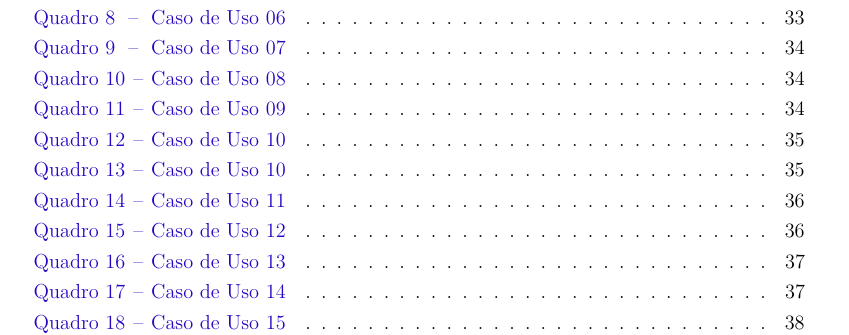
\includegraphics[width=0.9\textwidth]{exemplos/erros_lista_quadros.png}}
	\caption{\label{fig_erros_lista_quadros}Exemplo de Lista de quadros com erros comuns}
	\fonte{Trecho de um trabalho com o erro}
\end{figure}

\subsection{Erros em citações diretas}

A ABNT define formatos específicos para citações diretas, citações curtas e citações longas (mais de 3 linhas). A citação curta é feita diretamente durante a escrita do texto, mas a citação longa deve ser feita de uma forma especifica. A \autoref{fig_citacao_longa_errada} demonstra a forma errada da citação e a \autoref{fig_citacao_longa_certa} mostra o formato correto para a citação longa.

\begin{figure}[hb]
    \centering
\fbox{\begin{minipage}{\textwidth}
Podemos observar que historicamente existem problemas que devem ser tratados: 
    ``\lipsum[5]'' \cite{ETAL5}.
\end{minipage}}
    \caption{Citação direta longa - correta}
    \label{fig_citacao_longa_errada}
\end{figure}

\begin{figure}[hb]
    \centering
\fbox{\begin{minipage}{\textwidth}
Podemos observar que historicamente existem problemas que devem ser tratados: 
    \begin{citacao}
    \lipsum[5] \cite{ETAL5}.
    \end{citacao}
\end{minipage}}
    \caption{Citação direta longa - correta}
    \label{fig_citacao_longa_certa}
\end{figure}
